\chapter{Vision and Future Work}
\label{vision}

In this chapter we discuss a broader vision of embodied fabrication, expand on
the ideas presented so far, and present several possibilities for future
developments in our own work and for embodied fabrication more generally.
Crucially, the work presented in the preceding chapters need not be
taken as representative of embodied fabrication devices in terms of design,
functionality, or purpose. The devices we created, while giving birth to this
notion of embodied fabrication devices only cover a small swatch of the
potential landscape. To elucidate: we focused on novice designers (we could have
focused on experts or somewhere in between), we aimed our designs at
middle-school aged children (we could have aimed younger or older), we could
have focused more on inclusive design for those with physical and cognitive
disabilities, we focused on 3-dimensional design with 3D printing as the
fabrication output - one could have worked on ways to turn 2D designs into
3D-printable objects, or on flattening 3D files into slice forms suitable for a
laser cutter, or on embodied output for CNC machines, sewing machines and
e-textiles, or even standard shop tools for wood and metal. Some of these ideas
are already close to reality, as mentioned in the chapter on related work, and
if current trends in desktop fabrication continue, we will no doubt see other
possibilities arise.

Even in terms of constructing tangible interfaces for novice 3D design, we have
only scratched the surface. Indeed, we rejected many other possible designs in
choosing the physical format for our devices; the UCube, SnapCAD, and PopCAD,
while they may appear quite different (and are in many ways) they all operate
off of the same general paradigm: a set of vertical towers with actuators that
communicate integer coordinates via LEDs that connect to a piece of software
which takes care of most of the visualization and modeling algorithms. Although
we had some success with this formula, it is far from the only one we considered
(and of course there are many potential designs we failed to think of). While
working within the integer lattice on step-by-step, very intentional interfaces
provided some worthy advantages and a remarkable range of output considering the
restraints, one could have gone many other directions.

To provide a truncated list of the many ideas we had and suggestions we
received: various means by which to perturb the physical points off the integer
lattice, through sliders, potentiometers, force sensors, resistor networks,
etc.; using some sort of lateral connection or visualization to make horizontal
connections more apparent, by electroluminescent wire, e-textile strips, or
reflected light; to forgo the hardware and use a 3D camera, 3D scanner, or
mobile phone combined with computer vision techniques to read in real-world
objects, clay, or some other modeling material instead of switch states from a
device. We had our reasons for not implementing some of these (to avoid blocking
movement through the modeling space, the desire to maintain a tangible
interface) but that certainly does not mean that these ideas could be
implemented very effectively in other embodied fabrication devices. Indeed,
several of the limitations of our devices, noted earlier, could be resolved with
some of these different approaches - modeling curves, complex shapes with many
input points, geometric shapes off the integer lattice - and undoubtedly others
could think of even more innovative interfaces in this area.

\section{Short Term Improvements}

From these myriad ideas, we move on to discuss some of the more direct future
work that could be done with our devices. Starting with SnapCAD, then: given the
ability to relate different colors, and thus represent multiple shapes or
players, we have yet to really explore this area. We envision not just a
modeling apparatus, but a platform for 3D spatial interaction that goes well
beyond the ``tic-tac-toe'' and sample modeling game we discussed in chapter 2.
Additions could extend the number of players and colors to three, four, or five,
we can implement new modeling modes or functions that take advantage of multiple
shapes, such as taking the union, intersection, or difference of two or more
convex hulls. Additionally, the towers we designed originally do not need to be
the only ``input objects'' - one could imagine a number of different objects
also being able to slot in to the same interface, and depending on which object
the software was expecting, the software could change its behavior accordingly.
One might imagine towers that provided sonic feedback, and could take in and
replay audio samples, creating a sort of 3D spatial sequencer. One could outfit
towers with different sensors such as reed switches (which detect magnetism) -
thus giving the SnapCAD the ability to graph a point cloud representing the
strength of a particular magnet placed in the middle (or anywhere near) the
device.

As for PopCAD, given the different medium of the pop-up book (paper as opposed
to circuit boards), it is worth exploring the possibilities afforded by a
cheaper, more flexible material. To start with the obvious, our device could be
expanded to include a larger array of input points (5x5x5, say), we could
potentially find a way using tiny magnets or magnetic paint to achieve a similar
``snap'' effect as in SnapCAD, which would allow for the same kinds of multiple
color/player interactions discusses above. For instance, the flexibility of
paper might provide the means for new types of modeling actions. It is plausible
to imagine paper tabs or other mechanisms that perturb the LEDs off the integer
lattice, or alter the overall topology in such a way that new shapes are
possible (e.g. by deforming an equidistant grid into a spherical shape). A
deeper look into paper engineering and origami may yield some surprisingly
dynamic structures. These structures might be amenable to additional sensors or
hardware that could be embedded into the paper or the book to provide new
functionality (rotation, proximity, pressure). Additionally, due to the
inexpensive and portable nature of the PopCAD design, it is worth exploring the
sorts of interactions that could occur between several pop-up books (e.g.,
extending the input field to include two or more grids by ``snapping'' several
PopCADs together, networked interactions like cooperative modeling tasks, or
competitive games like 3D-battleship). By using paper as a material to think
with, we may find further possibilities as development continues. It is also
worth looking at redefining or expanding what ``paper'' means as a material and
what kinds of things can work with it. Although not yet available, there are
``circuit stickers'' made from a very thin and flexible substrate and designed
specifically to be used with paper, copper tape, and the like. While various
types of ``conductive paper'' are available, they are mostly designed for
custom scientific applications, and lack the sort of ``hackable'' potential that
a conductive paper for electronic paper-crafts would ideally have. Given that
paper can be made at home (or in a school lab or even classroom), it seems
likely that an electronics friendly recipe from the maker community before too
long. If a stencil-like method became available for finely separating conductive
and non-conductive elements while making a single sheet of paper, then we have
truly arrived at paper-based circuit boards. One can imagine a desktop 3D
printer being able to lay down thin layers of pulp in conductive and insulating
varieties to build, in-situ, a 3D paper circuit.

Due to its inexpensive nature, the PopCAD makes a good candidate for a DIY kit,
whereby the design files for the paper elements, the schematics for the
circuitry, and the harder-to-find components (like the fabric tape, LEDs, and
microcontroller) could all be packaged together and sold under an open source
license. As the democratization of technology is one of the goals of this work,
it seems fitting that an inexpensive, open-source kit be one of the results of
our research. Without including the paper, scissors, or soldering equipment, we
estimate that the components for a PopCAD kit would be roughly \$6US for the
LEDs, \$20 for the conductive tape, and \$30 for a microcontroller, for a total
of roughly \$60US with tac and shipping. \$60 may still prevent some educators
from purchasing a device, but certainly not as many as a \$500 device would.
With that in mind, we plan to redesign the PopCAD with a kit in mind - making
the circuit more straightforward and the construction more robust, while
developing solid documentation and instructions for distribution with the kit.

For the software, several less-fanciful or inspiring opportunities arise that
would nonetheless make significant improvements to the existing state of
affairs. The current software is written in Java, and as an application would
have to manually installed on any computer that wished to make use of it.
Porting the software to JavaScript and making use of new developments in HTML5
that greatly enhance a modern web browser's ability to display complex,
interactive 3D graphics would allow the application to be accessed from
anywhere. It has also become easier to connect peripherals attached to a home
computer to an application running in a web browser. There are many different
Ethernet shields available for Arduino, as well as the Arduino Yun, a single
board the combines an Arduino with a Linux-based operating system with WiFi and
Ethernet support. There is even a web-based integrated development environment
(IDE) for writing and uploading code onto an Arduino straight from a
browser\cite{CodeBender}. Combined, these methods would allow users all over the
world to run a local copy of the software, configure it for their own uses, and
receive and install the latest firmware versions of the Arduino code. There is
one advantage of the software currently being in Java, however - the Android
mobile operating system uses Java, so a mobile phone and tablet-based version of
the software could be made available with a little work, allowing those without
a desktop or laptop computer (or those who wanted to take a PopCAD camping with
them) to still make use of our contributions.

\begin{figure}[ht]
\begin{center}$
\begin{array}{cc}
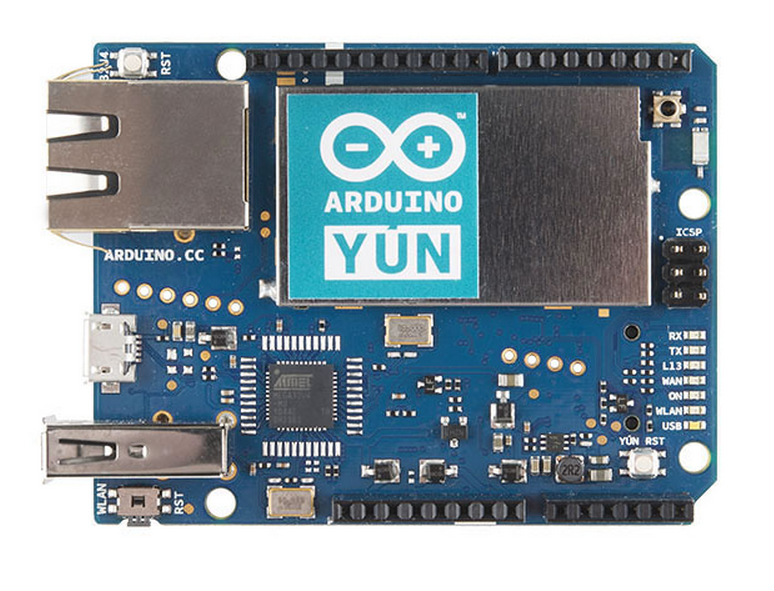
\includegraphics[width=.4\linewidth]{images/yun}&
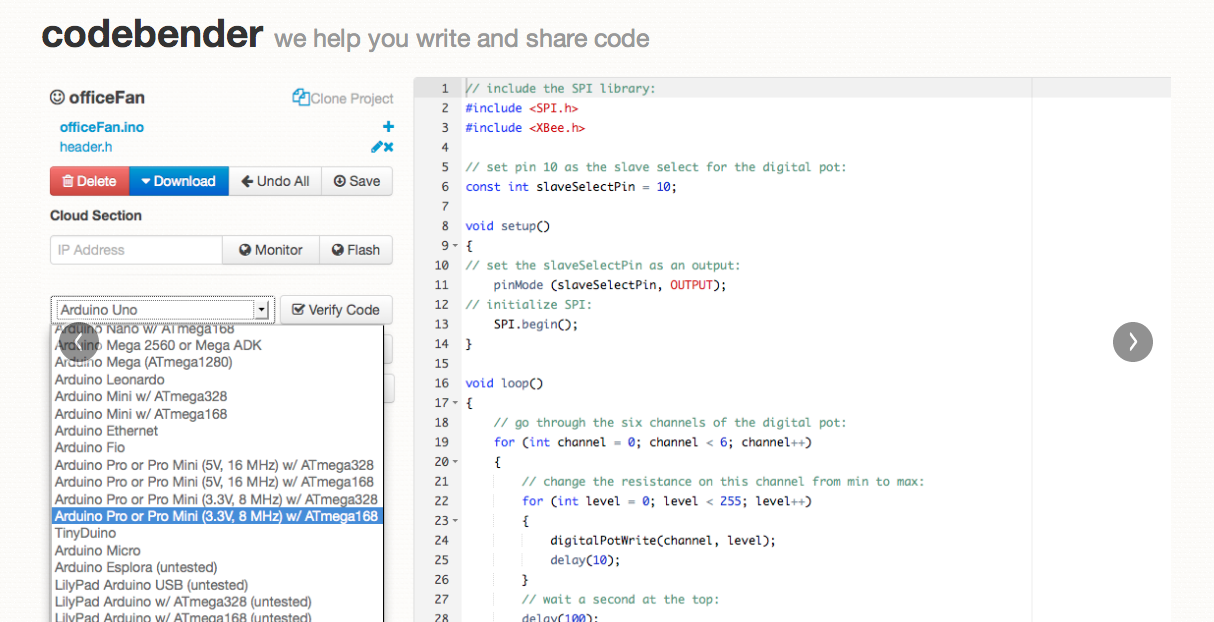
\includegraphics[width=.5\linewidth, height=2in]{images/codebender}
\end{array}$
\end{center}
\caption{Left: The Arduino Yun, an Arduino board with a Linux-based OS. Right:
codebender.cc, an open-source, web-based platform for writing and uploading
code directly to an Arduino.}
\label{yun}
\end{figure}

Additionally, we feel there is a fair amount still to explore in the video
footage we captured from the SnapCAD / PopCAD study. We recorded over 400 video
clips of participant modeling and 40 hours worth of screen capture from the
software during that time. We looked at modeling results and the gesture and
speech expressions made when answering a certain question about modeling, yet
there are many more things we could analyze given the time. For instance,
recording and coding the gestures made during the modeling process; does
gesturing while modeling correlate to modeling success, or to gesturing while
explaining modeling strategy? We could have done analysis on the screen capture
to see if subjects who interacted with the software more often were more likely
to be good modelers. We could look at the types of orientations the users put
the software in and detect any correlation between the amount of time spent in
certain orientations versus modeling success. These are questions we believe are
worth exploring, however the time and resources available to us have not allowed
such a thorough analysis to be completed.

\section{Extending Embodied Fabrication}

As we alluded to at the beginning of the chapter, the work we have presented is
but a minnow among whales compared to the potential work on embodied fabrication
research. We have given some concrete instances of improvements or changes that
could be made to our existing devices and software, without indicating (however
imperfectly) what might lay ahead for those interested in embodied fabrication
more generally. 

The core ideas in our work deal with creating means of increasing accessibility
to and understanding with emerging fabrication technology while maintaining a
sense of authorship and empowerment in the user, by leveraging the deep connections
between body and mind. These strands might be woven together in any number of
different ways and with greater emphasis on some aspects than others. By
breaking down these elements we might think intelligently about how focusing on
one of these might play out in relation to the rest. 

\begin{figure}[!ht]
\begin{center}$
\begin{array}{cc}
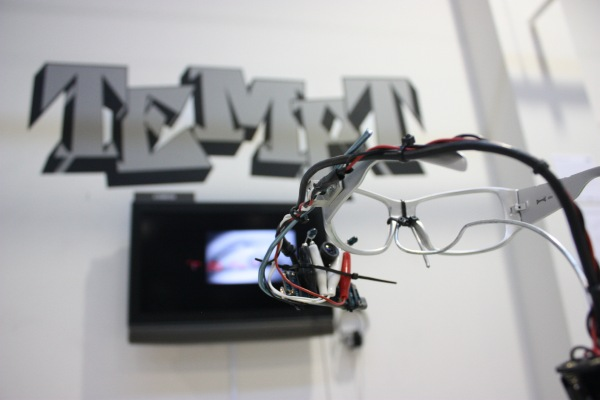
\includegraphics[width=.6\linewidth]{images/eyewriter}&
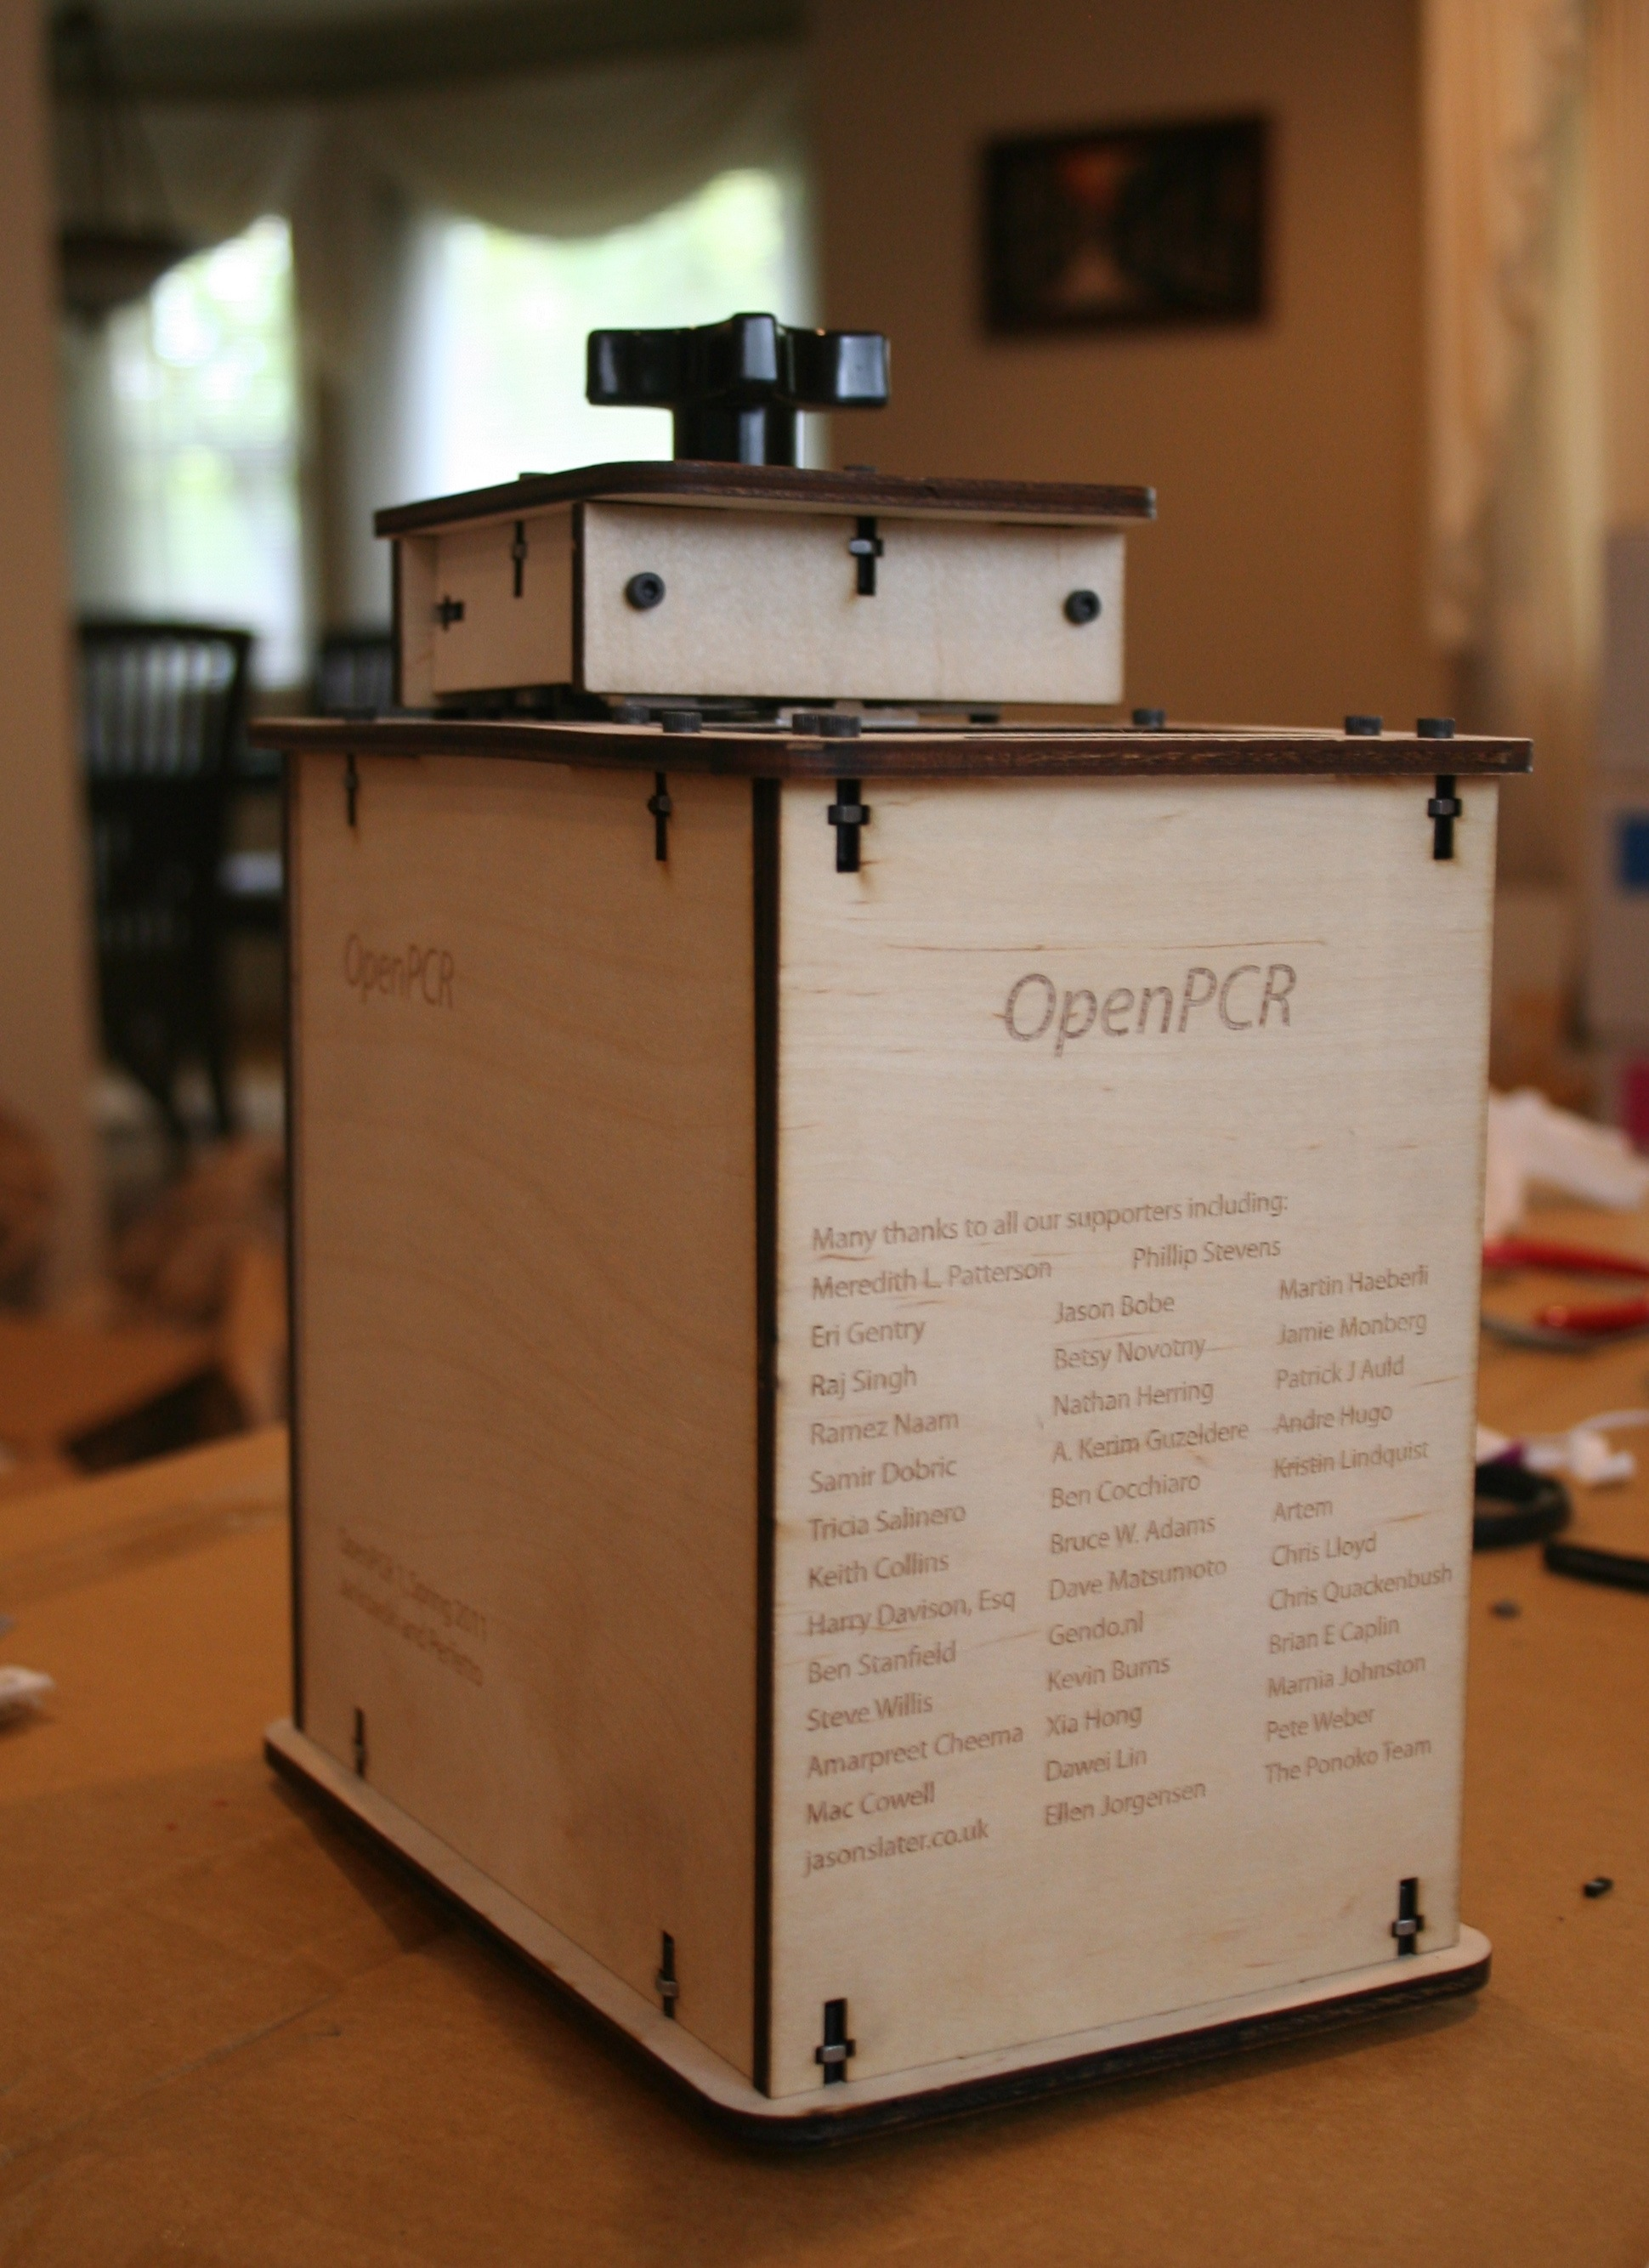
\includegraphics[width=.3\linewidth]{images/openPCR}
\end{array}$
\end{center}
\caption{Left: The EyeWriter, a wearable eye-tracking system connected to a
paint program that allows users with ALS (or other forms of paralysis) to
paint. Right: The OpenPCR, an affordable, open-source polymerase chain
reaction (PCR) machine that can be used at-home for DNA replication, gene
sequencing, and more.}
\label{eyewriter}
\end{figure}

In focusing on accessibility, we might envision devices created to give a
greater sense of 3D modeling to those with severe vision impairments, perhaps
with a combination of familiar materials such as clay or play-doh and wearable
haptic devices. We might think of ways to take input from those with limited
motor skills and transform it into potential output for 3D printers and laser
cutters - see for example the EyeWriter project\cite{EyeWriter} in which a group
of technologists developed a set of glasses for a former graffiti artist who had
been diagnosed with ALS (Lou Gehrig's disease) and only had free movement with
his eyes. The glasses would track eye movement and allow eye movements to
control a drawing program, allowing him to create artwork again. We can imagine
a similar set of devices for the creation of artifacts for 3D printing, laser
cutting, sewing, or even circuit design.

Another interesting thought comes from the DIY-biology movement, which has
released (and continues to work on) ways of creating affordable polymerase chain
reaction (PCR) machines, used for DNA replication, sequencing, and analysis. The
OpenPCR\cite{OpenPCR} is a completely open-source PCR machine currently
available for \$600 (a fraction of traditional lab versions, much like
industrial 3D printers). Imagine creating an embodied interface that teaches
children how DNA replication and gene sequencing works!

To summarize, while there are some concrete steps to take in our own work, the
vision for embodied fabrication devices, while incredibly exciting to think
about, is far too open at this stage to offer more than mere speculation. We can
only hope that other engineers, designers, artists, and scientists continue to
work on objects and technologies that spur others to create ways of
connecting their inventions to people in ways that inspire, empower, and
enlighten.

\section{Closing Remarks}

During the four years since beginning work on the first UCube prototype, our
thoughts and beliefs about the nature of our work evolved, became steadily more
focused and resulted in the work we present here on devices for embodied
fabrication. Over the course of designing three devices and three user studies,
we gained valuable insight into how young people think about 3D modeling, how they
interact with never-before-seen tangible devices, the kinds of models they
create, and the strategies they use (both verbal and gestural) to explain their
modeling decisions. This chapter is devoted to ``taking a look back'' at the
body of work that comprises this thesis and attempting to distill the most
relevant and unique findings into their most basic parts.

We have created three separate, fully-functional prototype devices, the UCube,
SnapCAD, and PopCAD, each of which interfaces with a piece of software (again,
that we created) that allows one to specify points in 3-space in various ways to
create 3-dimensional solids that can be easily exported into a 3D printable
format. We are aware of no other systems that combine the physical, embodied
nature of our designs with the express purpose of making design for 3D printing
accessible to novice designers as young as 11 years old.

We performed three separate user studies with over 50 hours of subject
interaction with our devices and over 40 different subjects, aged between 11-18
years old. Our first two studies showed that the UCube can be used to reproduce
convex hull models both from on-screen representations and from 3D printed
physical models. We also ran a matching task that strongly indicated that
children have the ability to mentally reconstruct and accurate convex hull from
a set of lighted points in 3-space. Our last study, a two-stage evaluation of
the PopCAD and SnapCAD, looked not only at convex hull performance, but at path
and minimal spanning tree modeling as well. Additionally, we had subjects do a
mental transformation exercise before and after the study to assess spatial
reasoning skills. We analyzed video recordings and coded the speech and gesture
expressions produced when participants were asked about their modeling strategy.
We observed improvements in each of the three modeling modes, improvements in
the mental transformation task scores, and an increase in speech and gesture
expressions from the first to second sessions. Most encouraging was the dramatic
improvement we observed from girls over the course of the study. We found
correlations between the types of gesture and speech produced and overall
modeling ability, and based on prior research, we concluded that subjects who
exhibit a high number of gestures that are classified as most relevant to the
task at hand are in fact the most likely to perform well on that given task.
Interestingly, we found only a modest correlation between age and performance,
while an analysis of performance against shape complexity found a more
significant correlation.

Perhaps most importantly, children were deeply engaged by the devices. They took
advantage of an open modeling session to create a wildly diverse set of objects,
many taking longer than the allotted time just to explore the possibilities of
the interface. This is crucial given the fact that the subjects in all three
studies were given very minimal instruction on how to use the device, and no
instruction on how to \emph{think} about the relationships between the physical
device and the software. The ability of the devices to engage youngsters in
exploratory play will allow them to come to their own conclusions about how to
operate the interfaces most effectively, and will no doubt lead to unforeseen
adaptations and use-cases. The engagement we witnessed indicates to us that an
interface such as the ones we have devised would likely be a welcome addition to
many educational spaces, and even some homes (many kids we worked with said they
``wanted one''). Is it our hope that this work will continue on in such a way as to
fulfill these children's wishes, with the creation of ever-more engaging,
expressive, and diverse tools that combine thinking with the mind and acting
with the body to bring a deeper level of understanding and learning to the full
breadth of human experience.

